% This file was created by tikzplotlib v0.9.1.
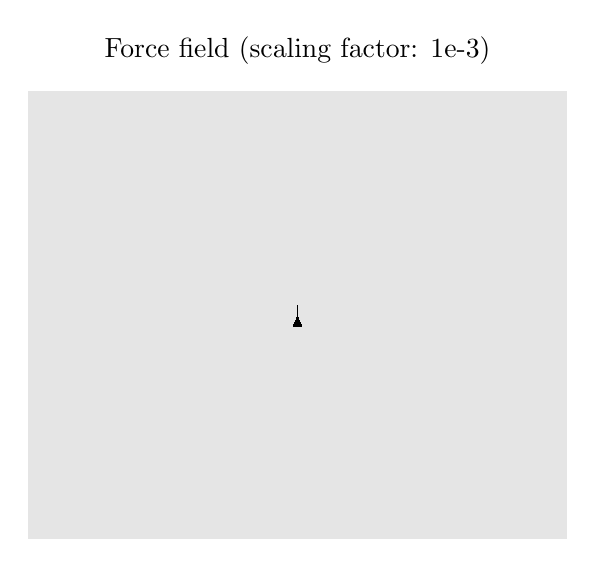
\begin{tikzpicture}

\begin{axis}[
axis background/.style={fill=white!89.8039215686275!black},
axis line style={white},
hide x axis,
hide y axis,
tick align=outside,
tick pos=left,
title={Force field (scaling factor: 1e-3)},
x grid style={white},
xlabel={x axis},
xmajorgrids,
xmin=-0.05, xmax=0.05,
xtick style={color=white!33.3333333333333!black},
y dir=reverse,
y grid style={white},
ylabel style={rotate=-90.0},
ylabel={y axis},
ymajorgrids,
ymin=-0.05, ymax=0.05,
ytick style={color=white!33.3333333333333!black}
]
\draw[-latex,draw=black] (axis cs:0,0) -- (axis cs:0,0);
\draw[-latex,draw=black] (axis cs:0,0) -- (axis cs:0,0);
\draw[-latex,draw=black] (axis cs:0,0) -- (axis cs:0,0);
\draw[-latex,draw=black] (axis cs:0,0) -- (axis cs:0,0);
\draw[-latex,draw=black] (axis cs:0,0) -- (axis cs:0,0);
\draw[-latex,draw=black] (axis cs:0,0) -- (axis cs:0,0);
\draw[-latex,draw=black] (axis cs:0,0) -- (axis cs:0,0);
\draw[-latex,draw=black] (axis cs:0,0) -- (axis cs:0,0);
\draw[-latex,draw=black] (axis cs:0,0) -- (axis cs:0,0);
\draw[-latex,draw=black] (axis cs:0,0) -- (axis cs:0,0);
\draw[-latex,draw=black] (axis cs:0,0) -- (axis cs:0,0);
\draw[-latex,draw=black] (axis cs:0,0) -- (axis cs:0,0);
\draw[-latex,draw=black] (axis cs:0,0) -- (axis cs:0,0);
\draw[-latex,draw=black] (axis cs:0,0) -- (axis cs:0,0);
\draw[-latex,draw=black] (axis cs:0,0) -- (axis cs:0,0);
\draw[-latex,draw=black] (axis cs:0,0) -- (axis cs:0,0);
\draw[-latex,draw=black] (axis cs:0,0) -- (axis cs:0,0);
\draw[-latex,draw=black] (axis cs:0,0) -- (axis cs:0,0);
\draw[-latex,draw=black] (axis cs:0,0) -- (axis cs:0,0);
\draw[-latex,draw=black] (axis cs:0,0) -- (axis cs:0,0);
\draw[-latex,draw=black] (axis cs:0,0) -- (axis cs:0,0);
\draw[-latex,draw=black] (axis cs:0,0) -- (axis cs:0,0);
\draw[-latex,draw=black] (axis cs:0,0) -- (axis cs:0,0);
\draw[-latex,draw=black] (axis cs:0,0) -- (axis cs:0,0);
\draw[-latex,draw=black] (axis cs:0,0) -- (axis cs:0,0);
\draw[-latex,draw=black] (axis cs:0,0) -- (axis cs:0,0);
\draw[-latex,draw=black] (axis cs:0,0) -- (axis cs:0,0);
\draw[-latex,draw=black] (axis cs:0,0) -- (axis cs:0,0);
\draw[-latex,draw=black] (axis cs:0,0) -- (axis cs:0,0);
\draw[-latex,draw=black] (axis cs:0,0) -- (axis cs:0,0);
\draw[-latex,draw=black] (axis cs:0,0) -- (axis cs:0,0);
\draw[-latex,draw=black] (axis cs:0,0) -- (axis cs:0,0);
\draw[-latex,draw=black] (axis cs:0,0) -- (axis cs:0,0);
\draw[-latex,draw=black] (axis cs:0,0) -- (axis cs:0,0);
\draw[-latex,draw=black] (axis cs:0,0) -- (axis cs:0,0);
\draw[-latex,draw=black] (axis cs:0,0) -- (axis cs:0,0);
\draw[-latex,draw=black] (axis cs:0,0) -- (axis cs:0,0);
\draw[-latex,draw=black] (axis cs:0,0) -- (axis cs:0,0);
\draw[-latex,draw=black] (axis cs:0,0) -- (axis cs:0,0);
\draw[-latex,draw=black] (axis cs:0,0) -- (axis cs:0,0);
\draw[-latex,draw=black] (axis cs:0,0) -- (axis cs:0,0);
\draw[-latex,draw=black] (axis cs:0,0) -- (axis cs:0,0);
\draw[-latex,draw=black] (axis cs:0,0) -- (axis cs:0,0);
\draw[-latex,draw=black] (axis cs:0,0) -- (axis cs:0,0);
\draw[-latex,draw=black] (axis cs:0,0) -- (axis cs:0,0);
\draw[-latex,draw=black] (axis cs:0,0) -- (axis cs:0,0);
\draw[-latex,draw=black] (axis cs:0,0) -- (axis cs:0,0);
\draw[-latex,draw=black] (axis cs:0,0) -- (axis cs:0,0);
\draw[-latex,draw=black] (axis cs:0,0) -- (axis cs:0,0);
\draw[-latex,draw=black] (axis cs:0,0) -- (axis cs:0,0);
\draw[-latex,draw=black] (axis cs:0,0) -- (axis cs:0,0);
\draw[-latex,draw=black] (axis cs:0,0) -- (axis cs:0,0);
\draw[-latex,draw=black] (axis cs:0,0) -- (axis cs:0,0);
\draw[-latex,draw=black] (axis cs:0,0) -- (axis cs:0,0);
\draw[-latex,draw=black] (axis cs:0,0) -- (axis cs:0,0);
\draw[-latex,draw=black] (axis cs:0,0) -- (axis cs:0,0);
\draw[-latex,draw=black] (axis cs:0,0) -- (axis cs:0,0);
\draw[-latex,draw=black] (axis cs:0,0) -- (axis cs:0,0);
\draw[-latex,draw=black] (axis cs:0,0) -- (axis cs:0,0);
\draw[-latex,draw=black] (axis cs:0,0) -- (axis cs:0,0);
\draw[-latex,draw=black] (axis cs:0,0) -- (axis cs:0,0);
\draw[-latex,draw=black] (axis cs:0,0) -- (axis cs:0,0);
\draw[-latex,draw=black] (axis cs:0,0) -- (axis cs:0,0);
\draw[-latex,draw=black] (axis cs:0,0) -- (axis cs:0,0);
\draw[-latex,draw=black] (axis cs:0,0) -- (axis cs:0,0);
\draw[-latex,draw=black] (axis cs:0,0) -- (axis cs:0,0);
\draw[-latex,draw=black] (axis cs:0,0) -- (axis cs:0,0);
\draw[-latex,draw=black] (axis cs:0,0) -- (axis cs:0,0);
\draw[-latex,draw=black] (axis cs:0,0) -- (axis cs:0,0);
\draw[-latex,draw=black] (axis cs:0,0) -- (axis cs:0,0);
\draw[-latex,draw=black] (axis cs:0,0) -- (axis cs:0,0);
\draw[-latex,draw=black] (axis cs:0,0) -- (axis cs:0,0);
\draw[-latex,draw=black] (axis cs:0,0) -- (axis cs:0,0);
\draw[-latex,draw=black] (axis cs:0,0) -- (axis cs:0,0);
\draw[-latex,draw=black] (axis cs:0,0) -- (axis cs:0,0);
\draw[-latex,draw=black] (axis cs:0,0) -- (axis cs:0,0);
\draw[-latex,draw=black] (axis cs:0,0) -- (axis cs:0,0);
\draw[-latex,draw=black] (axis cs:0,0) -- (axis cs:0,0);
\draw[-latex,draw=black] (axis cs:0,0) -- (axis cs:0,0);
\draw[-latex,draw=black] (axis cs:0,0) -- (axis cs:0,0);
\draw[-latex,draw=black] (axis cs:0,0) -- (axis cs:0,0);
\draw[-latex,draw=black] (axis cs:0,0) -- (axis cs:0,0);
\draw[-latex,draw=black] (axis cs:0,0) -- (axis cs:0,0);
\draw[-latex,draw=black] (axis cs:0,0) -- (axis cs:0,0);
\draw[-latex,draw=black] (axis cs:0,0) -- (axis cs:0,0);
\draw[-latex,draw=black] (axis cs:0,0) -- (axis cs:0,0);
\draw[-latex,draw=black] (axis cs:0,0) -- (axis cs:0,0);
\draw[-latex,draw=black] (axis cs:0,0) -- (axis cs:0,0);
\draw[-latex,draw=black] (axis cs:0,0) -- (axis cs:0,0);
\draw[-latex,draw=black] (axis cs:0,0) -- (axis cs:0,0);
\draw[-latex,draw=black] (axis cs:0,0) -- (axis cs:0,0);
\draw[-latex,draw=black] (axis cs:0,0) -- (axis cs:0,0);
\draw[-latex,draw=black] (axis cs:0,0) -- (axis cs:0,0);
\draw[-latex,draw=black] (axis cs:0,0) -- (axis cs:0,0);
\draw[-latex,draw=black] (axis cs:0,0) -- (axis cs:0,0);
\draw[-latex,draw=black] (axis cs:0,0) -- (axis cs:0,0);
\draw[-latex,draw=black] (axis cs:0,0) -- (axis cs:0,0);
\draw[-latex,draw=black] (axis cs:0,0) -- (axis cs:0,0);
\draw[-latex,draw=black] (axis cs:0,0) -- (axis cs:0,0);
\draw[-latex,draw=black] (axis cs:0,0) -- (axis cs:0,0);
\draw[-latex,draw=black] (axis cs:0,0) -- (axis cs:0,0);
\draw[-latex,draw=black] (axis cs:0,0) -- (axis cs:0,0);
\draw[-latex,draw=black] (axis cs:0,0) -- (axis cs:0,0);
\draw[-latex,draw=black] (axis cs:0,0) -- (axis cs:0,0);
\draw[-latex,draw=black] (axis cs:0,0) -- (axis cs:0,0);
\draw[-latex,draw=black] (axis cs:0,0) -- (axis cs:0,0);
\draw[-latex,draw=black] (axis cs:0,0) -- (axis cs:0,0);
\draw[-latex,draw=black] (axis cs:0,0) -- (axis cs:0,0);
\draw[-latex,draw=black] (axis cs:0,0) -- (axis cs:0,0);
\draw[-latex,draw=black] (axis cs:0,0) -- (axis cs:0,0);
\draw[-latex,draw=black] (axis cs:0,0) -- (axis cs:0,0);
\draw[-latex,draw=black] (axis cs:0,0) -- (axis cs:0,0);
\draw[-latex,draw=black] (axis cs:0,0) -- (axis cs:0,0);
\draw[-latex,draw=black] (axis cs:0,0) -- (axis cs:0,0);
\draw[-latex,draw=black] (axis cs:0,0) -- (axis cs:0,0);
\draw[-latex,draw=black] (axis cs:0,0) -- (axis cs:0,0);
\draw[-latex,draw=black] (axis cs:0,0) -- (axis cs:0,0);
\draw[-latex,draw=black] (axis cs:0,0) -- (axis cs:0,0);
\draw[-latex,draw=black] (axis cs:0,0) -- (axis cs:0,0);
\draw[-latex,draw=black] (axis cs:0,0) -- (axis cs:0,0);
\draw[-latex,draw=black] (axis cs:0,0) -- (axis cs:0,0);
\draw[-latex,draw=black] (axis cs:0,0) -- (axis cs:0,0);
\draw[-latex,draw=black] (axis cs:0,0) -- (axis cs:0,0);
\draw[-latex,draw=black] (axis cs:0,0) -- (axis cs:0,0);
\end{axis}

\end{tikzpicture}
